% Created 2021-04-26 Mon 21:55
% Intended LaTeX compiler: pdflatex
\documentclass[twocolumn]{article}
\usepackage[utf8]{inputenc}
\usepackage[T1]{fontenc}
\usepackage{graphicx}
\usepackage{grffile}
\usepackage{longtable}
\usepackage{wrapfig}
\usepackage{rotating}
\usepackage[normalem]{ulem}
\usepackage{amsmath}
\usepackage{textcomp}
\usepackage{amssymb}
\usepackage{capt-of}
\usepackage{hyperref}
\usepackage[margin=0.5in]{geometry}
\usepackage{pgfplots}
\author{Hee Hwang and Sudarshan Raghavan}
\date{\today}
\title{Tasks}
\hypersetup{
 pdfauthor={Hee Hwang and Sudarshan Raghavan},
 pdftitle={Tasks},
 pdfkeywords={},
 pdfsubject={},
 pdfcreator={Emacs 26.3 (Org mode 9.1.9)}, 
 pdflang={English}}
\begin{document}

\maketitle



\section{Datasets}
\label{sec:orgfa400ad}
ACL  : Citation Intent Classification\\
Hyper: HyperPartisan News Detection\\
RCT  : Randomized Controlled Trials

\subsection{Size of Datasets}
\label{sec:org8936ea8}
\begin{center}
\begin{tabular}{lrrrr}
\hline
Task & train & dev & test & Classes\\
\hline
ACL & 1688 & 114 & 139 & 6\\
\hline
Hyper & 516 & 64 & 65 & 2\\
\hline
RCT-sample & 500 & 30212 & 30135 & 5\\
\hline
RCT-20k & 180040 & 30212 & 30135 & 5\\
\hline
\end{tabular}
\end{center}

\subsection{Size of Augmented Data}
\label{sec:orga98a931}
\begin{center}
\begin{tabular}{rlll}
\hline
Max Score & ACL & Hyper & RCT\\
\hline
Baseline & 1688 (100\%) & 516 (100\%) & 500(100\%)\\
\hline
24 & 1746 (103\%) & 551 (106\%) & 686(137\%)\\
\hline
26 & 1815 (107\%) & 567 (109\%) & 831(166\%)\\
\hline
28 & 1981 (117\%) & 606 (117\%) & 1065(213\%)\\
\hline
30 & 2253 (133\%) & 656 (127\%) & 1484(296\%)\\
\hline
32 & 2842 (168\%) & 742 (143\%) & 2105(421\%)\\
\hline
34 & 3848 (227\%) & 911 (176\%) & 2952(590\%)\\
\hline
36 & 5819 (344\%) & 1127 (218\%) & 4196(839\%)\\
\hline
\end{tabular}
\end{center}


\section{Augmentation}
\label{sec:org2d144ed}


\subsection{Augmentation by Maximum Similarity Score}
\label{sec:org4df79da}
\begin{center}
\begin{tabular}{rrrr}
\hline
Max Score & ACL & Hyper & RCT\\
\hline
Baseline & 62.70 & 90.24 & 73.60\\
\hline
24 & \textbf{73.45} & \textbf{93.66} & 70.06\\
\hline
26 & 71.71 & 81.98 & 69.19\\
\hline
28 & 66.17 & 92.03 & 64.50\\
\hline
30 & 65.34 & 81.32 & 60.57\\
\hline
32 & 61.64 & 88.85 & 58.77\\
\hline
34 & 59.56 & 83.75 & 53.47\\
\hline
36 & 59.22 & 88.70 & 53.27\\
\hline
\end{tabular}
\end{center}




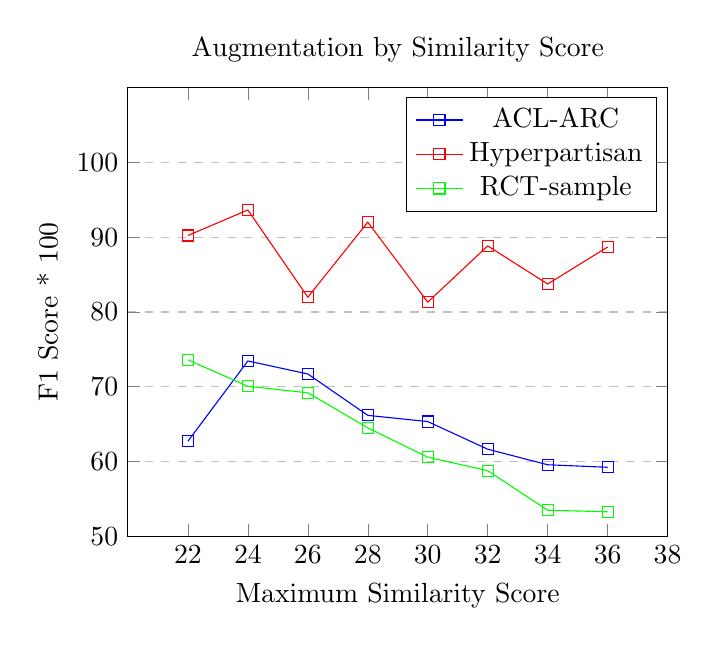
\begin{tikzpicture}
\begin{axis}[
    title={Augmentation by Similarity Score},
    xlabel={Maximum Similarity Score},
    ylabel={F1 Score * 100},
    xmin=20, xmax=38,
    ymin=50, ymax=110,
    xtick={22,24,26,28,30,32,34,36,38},
    ytick={50,60,70,80,90,100},
    ymajorgrids=true,
    grid style=dashed,
]
\addplot[ 
    color=blue, 
    mark=square, 
    ]
    coordinates {
    (22,62.70)(24,73.45)(26,71.71)(28,66.17)(30,65.34)(32,61.64)(34,59.56)(36,59.22)
    };
    \addlegendentry{ACL-ARC}

\addplot[
    color=red,
    mark=square,
    ]
    coordinates {
    (22,90.24)(24,93.66)(26,81.98)(28,92.03)(30,81.32)(32,88.85)(34,83.75)(36,88.70)
    };
    \addlegendentry{Hyperpartisan}

\addplot[
    color=green,
    mark=square,
    ]
    coordinates {
    (22,73.60)(24,70.06)(26,69.19)(28,64.50)(30,60.57)(32,58.77)(34,53.47)(36,53.27)
    };
    \addlegendentry{RCT-sample}

\end{axis}
\end{tikzpicture}


\section{Baseline models:}
\label{sec:org3f01150}
\begin{itemize}
\item An off-the-shelf RoBERTa model that has been finetuned to perform classification for each of the downstream tasks
\end{itemize}

\section{Augmentation Model}
\label{sec:orgee4db84}
\begin{center}
\includegraphics[width=.9\linewidth]{./png/da.png}
\end{center}


\section{Algorithm}
\label{sec:orgb9d0136}
\begin{verbatim}
1. Extract failed test examples from the baseline model
2. Retrieve passages/sentences from Common Crawl 
3. Apply augmentation strategy (i)-(iii)
4. Augment all the labelled CC data to the training data
5. Retrain RoBERTa on the augmented training set 
\end{verbatim}

\section{Augmentation Strategies}
\label{sec:orge5aa177}
\begin{itemize}
\item Strategy (i)\\
Use baseline model (Teacher) to perform unsupervised labelling on retrieved CC data
\item Strategy (ii)\\
Using a task specific binary classifier, 
filter out retrieved CC data that is "out-domain"\\
Use baseline model (Teacher) to perform unsupervised labelling on the filtered "in-domain" CC data
\item Strategy (iii)\\
Using a task specific binary classifier, 
filter out retrieved CC data that is "out-domain"\\
Use ground truth labels of failed test examples and assign labels to the filtered "in-domain" CC data
\end{itemize}
\end{document}
